\documentclass[12pt, a4paper]{article}

% Paquetes esenciales para matemáticas y formato
\usepackage[utf8]{inputenc}
\usepackage[spanish]{babel}
\usepackage{amsmath, amssymb, amsthm} % Para fórmulas matemáticas
\usepackage{geometry} % Para ajustar márgenes
\geometry{a4paper, margin=2.5cm}
\usepackage{tcolorbox}
\usepackage{graphicx} % Para insertar imágenes
\usepackage{xcolor}   % Para dar color a notas, dudas y código
\usepackage{listings} % Para insertar código fuente
\usepackage{hyperref} % Para enlaces clicables (se carga el último)

% Configuración del código Python
% (acepta tildes y eñes sin dar errores de compilación)
\lstset{
    language=Python,
    basicstyle=\small\ttfamily,
    backgroundcolor=\color{gray!10},
    frame=single,
    rulecolor=\color{black!30},
    keywordstyle=\color{blue}\bfseries,
    commentstyle=\color{green!50!black}\itshape,
    stringstyle=\color{orange},
    showstringspaces=false,
    breaklines=true,
    inputencoding=utf8,
    extendedchars=true,
    literate={á}{{\'a}}1 {é}{{\'e}}1 {í}{{\'i}}1 {ó}{{\'o}}1 {ú}{{\'u}}1 {ñ}{{\~n}}1 {Á}{{\'A}}1 {É}{{\'E}}1 {Í}{{\'I}}1 {Ó}{{\'O}}1 {Ú}{{\'U}}1 {Ñ}{{\~N}}1
}

% Configuración de los enlaces
\hypersetup{
    colorlinks=true,
    linkcolor=blue,
    filecolor=magenta,
    urlcolor=cyan,
    pdftitle={Cuaderno TFG - SVM y Cuántica},
}

\title{\textbf{Cuaderno de Investigación: TFG}\\ \large Aprendizaje Automático aplicado a Programación Cuántica}
\author{Elia Torres Simón \\ \small Tutor: Luis Fernando Llana Díaz}
\date{\today}

\begin{document}

\maketitle

\tableofcontents
\newpage

%=====================================================================
\section*{Hoja de Ruta del TFG}
\addcontentsline{toc}{section}{Hoja de Ruta del TFG}
%=====================================================================

\noindent Esta sección es la brújula del trabajo: qué estoy haciendo, qué llevo, qué falta y por dónde seguir. Hay que actualizarla a medida que se avance.

\subsection*{1. En qué consiste el trabajo}

\noindent El hilo conductor del TFG es la siguiente observación:

\begin{tcolorbox}[colback=teal!5!white,colframe=teal!75!black,title=\textbf{Idea central}]
Una SVM solo necesita saber calcular \textbf{productos escalares} entre los datos (el kernel). Un ordenador cuántico es, de forma natural, una máquina que calcula productos escalares entre estados de un espacio de Hilbert de dimensión $2^n$. Combinando ambas ideas se obtienen los \textbf{métodos de kernel cuántico} (\textit{Quantum Support Vector Machines}, QSVM).
\end{tcolorbox}

\noindent El método funciona en tres pasos:
\begin{enumerate}
    \item \textbf{Codificación (mapa de características cuántico).} Cada dato $\mathbf{x} \in \mathbb{R}^d$ se codifica en un estado de $n$ qubits mediante un circuito parametrizado por el propio dato:
    \[ |\phi(\mathbf{x})\rangle = U(\mathbf{x})\,|0\rangle^{\otimes n}. \]
    El circuito $U(\mathbf{x})$ desempeña el papel del mapa $\phi$ de la sección de kernels, con $\mathcal{H} = \mathbb{C}^{2^n}$.

    \item \textbf{Kernel cuántico.} Se define el kernel como el solapamiento (fidelidad) entre los estados:
    \[ K(\mathbf{x}, \mathbf{y}) = |\langle \phi(\mathbf{x}) \,|\, \phi(\mathbf{y}) \rangle|^2 = \big|\langle 0 |\, U(\mathbf{x})^\dagger U(\mathbf{y}) \,| 0 \rangle\big|^2. \]
    Se estima en el ordenador cuántico (o en un simulador) aplicando $U(\mathbf{y})$ y después $U(\mathbf{x})^\dagger$, midiendo, y contando la frecuencia con la que se obtiene el resultado $0\cdots0$.

    \item \textbf{Clasificación.} La matriz de Gram $K_{ij} = K(\mathbf{x}_i, \mathbf{x}_j)$ se introduce en el problema dual de la SVM, exactamente igual que un kernel clásico. La optimización sigue siendo \textbf{clásica y convexa}; lo cuántico solo interviene en el cálculo de $K$.
\end{enumerate}

\noindent \textbf{Estructura del trabajo (la historia que cuenta):}
\[
\text{SVM clásica} \;\rightarrow\; \text{Kernels} \;\rightarrow\; \text{Fundamentos cuánticos} \;\rightarrow\; \text{Kernels cuánticos} \;\rightarrow\; \text{Experimentos} \;\rightarrow\; \text{Limitaciones}
\]

\noindent \textbf{Contenido matemático propio a desarrollar:} demostrar que el kernel cuántico es siempre un kernel válido (semidefinido positivo). Pista: escribiendo $\rho(\mathbf{x}) = |\phi(\mathbf{x})\rangle\langle\phi(\mathbf{x})|$ se tiene
\[ K(\mathbf{x}, \mathbf{y}) = \mathrm{Tr}\big[\rho(\mathbf{x})\,\rho(\mathbf{y})\big] = \langle \rho(\mathbf{x}), \rho(\mathbf{y}) \rangle_{HS}, \]
es decir, un producto escalar (de Hilbert--Schmidt) en el espacio de matrices, lo que encaja directamente con la definición de kernel de la Sección 1.

\noindent \textbf{Referencias clave:} Havlíček et al. (2019) \cite{havlicek2019supervised}, que propone el método y lo ejecuta en hardware de IBM; Schuld y Killoran (2019) \cite{schuld2019quantum}, que da el marco teórico de ``espacios de características cuánticos''.

\subsection*{2. Estado actual}

\begin{tcolorbox}[colback=green!5!white,colframe=green!50!black,title=\textbf{Hecho}]
\textbf{Teoría:}
\begin{itemize}
    \item SVM completa: hiperplano, margen, problema primal, dualidad, condiciones KKT, vectores de soporte.
    \item Truco del núcleo: kernels, caracterización (Moore--Aronszajn / Mercer), convexidad del dual.
    \item Margen suave: variables de holgura, Hinge Loss, descenso de subgradiente.
\end{itemize}
\textbf{Código:}
\begin{itemize}
    \item SVM lineal primal (margen suave) por descenso de subgradiente, con el dataset de billetes.
    \item SVM dual (margen duro) resuelta con \texttt{scipy} respetando todas las restricciones, con Iris.
\end{itemize}
\end{tcolorbox}

\begin{tcolorbox}[colback=yellow!5!white,colframe=orange!75!black,title=\textbf{Empezado}]
\begin{itemize}
    \item Fundamentos cuánticos de \textbf{un solo sistema}: estados, qubits, medición (regla de Born), puertas unitarias de un qubit.
\end{itemize}
\end{tcolorbox}

\begin{tcolorbox}[colback=red!5!white,colframe=red!60!black,title=\textbf{Falta}]
\textbf{Teoría (parte clásica, SVM):}
\begin{itemize}
    \item \textbf{Dual del margen suave} (prioritario): derivación completa, que lleva a las cotas $0 \le \alpha_i \le C$. Interpretación KKT de los tres casos: $\alpha_i = 0$ (bien clasificado, fuera del margen), $0 < \alpha_i < C$ (sobre el margen; son los que se usan para calcular $b$) y $\alpha_i = C$ (dentro del margen o mal clasificado). Es la formulación que usará la QSVM.
    \item Función de decisión con kernel, $f(\mathbf{x}) = \sum_i \alpha_i y_i K(\mathbf{x}_i, \mathbf{x}) + b$, y cálculo de $b$ con kernel.
    \item Evaluación de modelos: división entrenamiento/prueba, precisión, validación cruzada para elegir $C$ y $\gamma$.
    \item \textit{Opcional:} teorema del representante y espacios de Hilbert con núcleo reproductor (RKHS).
\end{itemize}
\textbf{Teoría (parte cuántica):}
\begin{itemize}
    \item Sistemas de varios qubits: producto tensorial, estados producto y entrelazados, puertas de varios qubits (CNOT, controladas).
    \item Circuitos cuánticos y medición de varios qubits.
    \item Codificación de datos en estados cuánticos: codificación por ángulos, \texttt{ZZFeatureMap}.
    \item Kernel cuántico: definición, estimación por medidas, error por número finito de disparos (\textit{shots}), demostración de que es semidefinido positivo.
    \item Limitaciones: concentración exponencial de los valores del kernel al crecer el número de qubits \cite{thanasilp2024exponential}, y en qué casos hay ventaja cuántica demostrada \cite{liu2021rigorous}.
\end{itemize}
\textbf{Código y práctica (parte clásica, SVM):}
\begin{itemize}
    \item SVM dual de \textbf{margen suave} con kernel genérico: cotas \texttt{(0, C)} en lugar de \texttt{(0, None)} y una función que reciba cualquier matriz $K$. Probarla con kernel lineal y RBF.
    \item Función \texttt{predecir} para puntos nuevos y separación entrenamiento/prueba con medida de precisión.
    \item Comprobar la implementación contra \texttt{sklearn.svm.SVC}: mismos $\alpha$, $b$ y predicciones.
    \item Estandarizar los datos (centrar y escalar) antes de entrenar. Importante para RBF y, sobre todo, para el kernel cuántico, donde los datos se codifican como ángulos.
\end{itemize}
\textbf{Código y práctica (parte cuántica):}
\begin{itemize}
    \item Primeros pasos en Qiskit: construir circuitos, simular, medir.
    \item Calcular la matriz del kernel cuántico con Qiskit (primero a mano con circuitos propios, después con \texttt{FidelityQuantumKernel} de \texttt{qiskit-machine-learning} para comprobar).
    \item Introducir el kernel cuántico en la SVM dual propia y clasificar.
    \item Experimentos comparativos (ver Fase 3).
\end{itemize}
\end{tcolorbox}

\subsection*{3. Plan de trabajo}

\paragraph{Fase 1 (octubre): base cuántica, Qiskit y cierre de la parte SVM.}\mbox{}
\begin{itemize}
    \item \textbf{Curso de IBM:} terminar los bloques de \textit{sistemas múltiples} y \textit{circuitos cuánticos}, pasándolos a este cuaderno igual que la parte de un solo sistema.
    \item \textbf{Qiskit:} instalarlo y reproducir los ejemplos básicos: estados de Bell, medición, histogramas de resultados.
    \item \textbf{Teoría SVM:} derivar el dual del margen suave con su interpretación KKT, escribir la función de decisión con kernel y añadir la metodología de evaluación (entrenamiento/prueba, validación cruzada).
    \item \textbf{Código SVM:} SVM dual de margen suave con kernel genérico, función de predicción, estandarización de datos y comprobación contra \texttt{sklearn.svm.SVC}. Probarla con RBF en un dataset no separable linealmente (por ejemplo, \texttt{make\_circles} o \texttt{make\_moons} de \texttt{sklearn}).
\end{itemize}
\textit{Resultado esperado:} entender un circuito de varios qubits y tener un solver de SVM de margen suave, validado, ``enchufable'' a cualquier kernel.

\paragraph{Fase 2 (noviembre): kernels cuánticos.}\mbox{}
\begin{itemize}
    \item \textbf{Teoría:} codificación de datos, definición del kernel de fidelidad, circuito de estimación ($U(\mathbf{y})$ seguido de $U(\mathbf{x})^\dagger$), error estadístico por número de disparos, demostración de la semidefinición positiva.
    \item \textbf{Código:} implementar un feature map sencillo (codificación por ángulos) y otro con entrelazamiento (\texttt{ZZFeatureMap}); calcular la matriz $K$ y resolver la SVM dual con ella.
    \item Comprobación: comparar la $K$ propia con la de \texttt{FidelityQuantumKernel}.
\end{itemize}
\textit{Resultado esperado:} una QSVM funcionando de principio a fin, con código propio en la parte de optimización.

\paragraph{Fase 3 (diciembre): experimentos y limitaciones.}\mbox{}
\begin{itemize}
    \item \textbf{Comparativa:} kernel lineal vs.\ RBF vs.\ kernels cuánticos en datasets pequeños (Iris, billetes con 2--4 variables, y un dataset ``de juguete'' diseñado para favorecer al kernel cuántico, como el \textit{ad hoc} de Havlíček et al.). Medir precisión en entrenamiento y test.
    \item \textbf{Efecto de los disparos:} cómo cambian la matriz $K$ y la precisión con 100, 1000, 10000 \textit{shots}.
    \item \textbf{Concentración:} observar numéricamente cómo los valores de $K$ se concentran al aumentar el número de qubits.
    \item \textbf{Opcional:} simulación con ruido, o ejecución en hardware real de IBM si el tutor lo considera interesante.
\end{itemize}
\textit{Resultado esperado:} resultados y figuras para la memoria, y una conclusión honesta sobre cuándo aporta algo lo cuántico.

\subsection*{4. Próximos pasos inmediatos (hasta la reunión del 2 de octubre)}

\begin{enumerate}
    \item \textbf{Leer el resumen y la introducción de Havlíček et al.} \cite{havlicek2019supervised}. La lectura completa se deja para la Fase 2.
    \item \textbf{Curso de IBM: sistemas múltiples} (prioridad de la semana), pasándolo a este cuaderno.
    \item \textbf{Tareas pendientes:} regenerar \texttt{diagrama2.png} con el nuevo código del dual y completar \texttt{referencias.bib}.
    \item \textbf{Leer la declaración responsable sobre autoría y uso ético de herramientas de IA} de la facultad (página de TFG de matematicas.ucm.es).
    \item \textbf{Preparar la reunión:}
    \begin{itemize}
        \item Explicar la idea en un minuto sin leer: SVM con kernels cuánticos; la SVM solo necesita productos escalares, así que el kernel se calcula con un circuito y la optimización sigue siendo clásica; implementación propia, comparación con kernels clásicos y limitaciones.
        \item Preguntas: normativa y plantilla de la facultad, extensión esperada; fecha límite de depósito para febrero; hardware real o simulador.
    \end{itemize}
\end{enumerate}

\subsection*{5. Cómo llegué al tema}

\begin{enumerate}
    \item Al derivar el dual de la SVM (Sección 1) vi que el problema y la función de decisión dependen de los datos solo a través de productos escalares, lo que lleva al truco del núcleo y a los espacios de características (\textit{feature spaces}).
    \item Buscando en Google Scholar ``quantum support vector machine'' encontré la propuesta original de SVM cuántica, Rebentrost, Mohseni y Lloyd (2014) \cite{rebentrost2014quantum}, cuya ventaja se basa en evaluar productos escalares con un ordenador cuántico. Ese enfoque resuelve toda la SVM en el ordenador cuántico y requiere hardware tolerante a fallos.
    \item Buscando ``feature spaces'' entre los artículos que citan a Rebentrost et al.\ encontré Havlíček et al.\ (2019) \cite{havlicek2019supervised}, donde el ordenador cuántico solo calcula el kernel y el resto es una SVM clásica, lo que lo hace viable en los ordenadores cuánticos actuales. Ese es el enfoque de este trabajo.
\end{enumerate}

\noindent \textbf{Método de trabajo con el tutor:} llevar a cada reunión algo concreto y acotado que validar (un resultado, una sección, una decisión), en lugar de preguntas abiertas.

\newpage

%=====================================================================
\section{Support Vector Machines (SVM): Conceptos Básicos}
%=====================================================================
\noindent \textbf{Vídeo}: \href{https://www.youtube.com/watch?v=39fx4h2uJNg}{Support Vector Machine (SVM) Intuition - Learn Machine Learning}

\noindent Intuición según el vídeo consultado: la clave de las SVM es que no se centran en los casos ``típicos'' de cada clase, sino en los casos extremos (los vectores de soporte) que están más cerca de la frontera de decisión. Esto lo hace un algoritmo muy robusto para encontrar el margen máximo.

\begin{figure}[htbp]
    \centering
    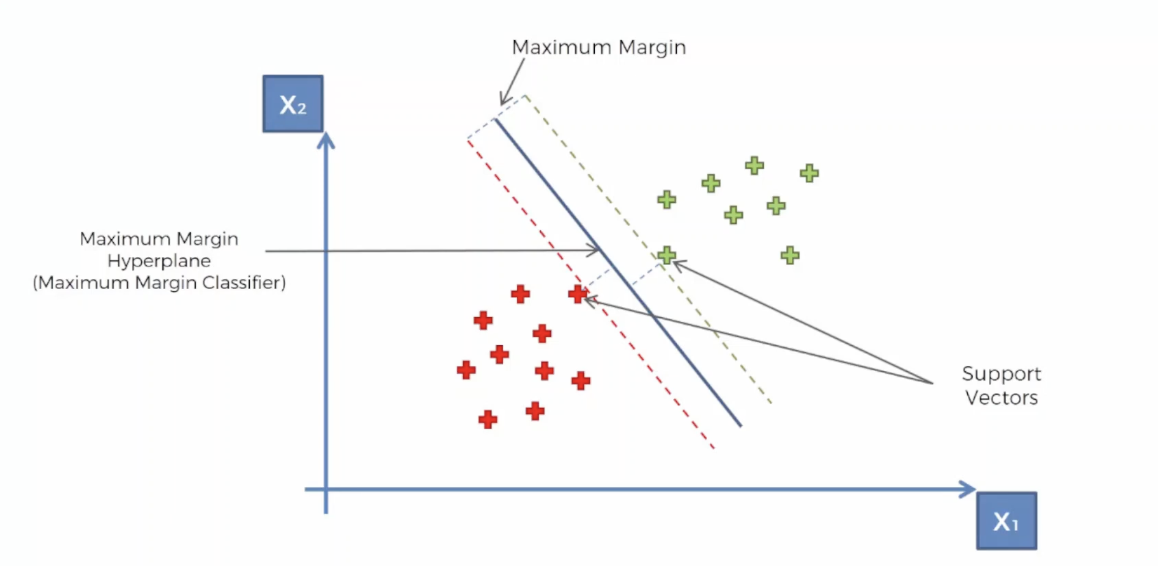
\includegraphics[width=0.8\textwidth]{diagrama.png}
    \caption{Representación geométrica de una SVM lineal. Se muestra el hiperplano separador ($=0$), los bordes del margen ($\pm 1$), el ancho del margen total $\frac{2}{\|\mathbf{w}\|}$ y los vectores de soporte que definen la frontera.}
    \label{fig:svm_diagrama}
\end{figure}

\subsection{Introducción y Definición Formal}
\noindent Las Máquinas de Vectores de Soporte (SVM) son un conjunto de algoritmos de aprendizaje supervisado desarrollados por Vapnik y colaboradores \cite{cortes1995support}. Formalmente, dado un conjunto de entrenamiento de $n$ puntos de la forma:
\[ \mathcal{D} = \{(\mathbf{x}_i, y_i) \mid \mathbf{x}_i \in \mathbb{R}^d, y_i \in \{-1, 1\}\}_{i=1}^n \]
donde $y_i$ indica la clase a la que pertenece el vector de características $\mathbf{x}_i$, el objetivo de una SVM es encontrar el \textbf{hiperplano separador de margen máximo}.

\subsection{El Hiperplano Separador}
\noindent Un hiperplano en $\mathbb{R}^d$ se define mediante la ecuación:
\[ f(\mathbf{x}) = \mathbf{w}^T \mathbf{x} + b = 0 \]
donde:
\begin{itemize}
    \item $\mathbf{w} \in \mathbb{R}^d \setminus \{\mathbf{0}\}$ es el vector normal al hiperplano (determina su orientación).
    \item $b \in \mathbb{R}$ es el sesgo o \textit{bias} (determina el desplazamiento desde el origen).
\end{itemize}

\noindent El par $(\mathbf{w}, b)$ no es único: $(c\mathbf{w}, cb)$ define el mismo hiperplano para todo $c > 0$. Fijamos esta libertad con la \textbf{normalización canónica}: escalamos $(\mathbf{w}, b)$ de modo que los puntos más cercanos al hiperplano cumplan $|\mathbf{w}^T \mathbf{x}_i + b| = 1$. Con esta normalización, para un conjunto linealmente separable buscamos un hiperplano tal que para todo $i$:
\[ y_i(\mathbf{w}^T \mathbf{x}_i + b) \geq 1 \]

\begin{tcolorbox}[colback=blue!5!white,colframe=blue!75!black,title=\textbf{Nota Aclaratoria: Entendiendo la inecuación del margen}]
La inecuación $y_i(\mathbf{w}^T \mathbf{x}_i + b) \geq 1$ es el núcleo de la SVM porque condensa tres ideas geométricas en una sola línea:

\textbf{1. La frontera (El 0):}\\
El hiperplano central es $\mathbf{w}^T \mathbf{x} + b = 0$. Si evaluamos un punto $\mathbf{x}_i$ en esta expresión, el resultado será positivo si está a un lado del hiperplano, y negativo si está al otro.

\textbf{2. El truco del signo ($y_i$):}\\
Como nuestras clases están etiquetadas como $+1$ y $-1$, al multiplicar la evaluación del punto por su etiqueta real ($y_i$), unificamos la condición de éxito.
\begin{itemize}
    \item Clase $+1$ en lado positivo: $(+1) \cdot (+) = +$
    \item Clase $-1$ en lado negativo: $(-1) \cdot (-) = +$
\end{itemize}
Por tanto, para clasificar correctamente, bastaría con exigir que $y_i(\mathbf{w}^T \mathbf{x}_i + b) > 0$.

\textbf{3. La zona de seguridad (El 1):}\\
La SVM no solo quiere clasificar bien, quiere \textit{maximizar el margen}. Al cambiar el $> 0$ por un $\geq 1$ (lo cual, gracias a la normalización canónica, no supone pérdida de generalidad), estamos forzando la creación de una ``calle'' de seguridad. Ningún punto puede invadir la zona entre $-1$ y $1$. Los puntos que cumplen la igualdad ($=1$) son los que están rozando el límite de la calle: los \textbf{Vectores de Soporte}.
\end{tcolorbox}

\subsection{Maximización del Margen}
\noindent El \textbf{margen geométrico} se define como la distancia entre el hiperplano y los puntos más cercanos de cada clase. Con la normalización canónica, esta distancia es $\frac{1}{\|\mathbf{w}\|}$ \cite{hastie2009elements}. Por lo tanto, el margen total entre las dos clases es $\frac{2}{\|\mathbf{w}\|}$.

\begin{tcolorbox}[colback=gray!5!white,colframe=gray!75!black,title=\textbf{Demostración: Cálculo del margen geométrico}]
Queremos calcular la distancia entre los dos hiperplanos que definen el margen:
\begin{enumerate}
    \item $H_1: \mathbf{w}^T \mathbf{x} + b = 1$
    \item $H_2: \mathbf{w}^T \mathbf{x} + b = -1$
\end{enumerate}

Sea $\mathbf{x}_1$ un punto en $H_1$ y $\mathbf{x}_2$ un punto en $H_2$. El vector $(\mathbf{x}_1 - \mathbf{x}_2)$ une ambos hiperplanos, pero no necesariamente de forma perpendicular. La distancia perpendicular (el margen $M$) es la \textbf{proyección} de este vector sobre el vector normal unitario del hiperplano.

El vector normal al hiperplano es $\mathbf{w}$, por lo que el vector normal unitario es $\hat{\mathbf{n}} = \frac{\mathbf{w}}{\|\mathbf{w}\|}$.

La distancia $M$ viene dada por el producto escalar:
\[ M = (\mathbf{x}_1 - \mathbf{x}_2)^T \frac{\mathbf{w}}{\|\mathbf{w}\|} = \frac{\mathbf{w}^T \mathbf{x}_1 - \mathbf{w}^T \mathbf{x}_2}{\|\mathbf{w}\|} \]

Como $\mathbf{x}_1 \in H_1$, sabemos que $\mathbf{w}^T \mathbf{x}_1 = 1 - b$. \\
Como $\mathbf{x}_2 \in H_2$, sabemos que $\mathbf{w}^T \mathbf{x}_2 = -1 - b$.

Sustituyendo en la ecuación de la distancia:
\[ M = \frac{(1 - b) - (-1 - b)}{\|\mathbf{w}\|} = \frac{2}{\|\mathbf{w}\|} \]

Por lo tanto, la distancia total del margen es $\frac{2}{\|\mathbf{w}\|}$, y la distancia desde el hiperplano central ($\mathbf{w}^T \mathbf{x} + b = 0$) a cualquiera de los bordes es la mitad: $\gamma = \frac{1}{\|\mathbf{w}\|}$.

\textit{Referencia: resultado estándar de geometría afín aplicado a la SVM \cite{hastie2009elements, bishop2006pattern}.}
\end{tcolorbox}

\noindent Maximizar el margen $\frac{2}{\|\mathbf{w}\|}$ es equivalente a minimizar $\frac{1}{2}\|\mathbf{w}\|^2$.

\begin{tcolorbox}[colback=blue!5!white,colframe=blue!75!black,title=\textbf{Nota Aclaratoria: ¿Por qué minimizamos $\frac{1}{2}\|\mathbf{w}\|^2$?}]

\textbf{1. Invertir la fracción (de maximizar a minimizar):}\\
Como $\mathbf{w} \neq \mathbf{0}$, la norma $\|\mathbf{w}\|$ es estrictamente positiva. Maximizar $\frac{2}{\|\mathbf{w}\|}$ equivale a minimizar $\|\mathbf{w}\|$ (el 2 del numerador es una constante y no afecta a dónde se alcanza el óptimo).

\textbf{2. Elevar al cuadrado (para quitar la raíz):}\\
Como $t \mapsto t^2$ es estrictamente creciente en $[0, \infty)$, minimizar $\|\mathbf{w}\|$ es lo mismo que minimizar $\|\mathbf{w}\|^2$: el minimizador es el mismo. La ventaja es que $\|\mathbf{w}\| = \sqrt{w_1^2 + \dots + w_d^2}$ no es diferenciable en el origen y su gradiente es más engorroso, mientras que $\|\mathbf{w}\|^2$ es una función cuadrática, convexa y diferenciable en todo punto.

\textbf{3. Multiplicar por $\frac{1}{2}$ (por comodidad):}\\
El gradiente de $\|\mathbf{w}\|^2$ es $2\mathbf{w}$. Con el factor $\frac{1}{2}$, el gradiente queda simplemente $\mathbf{w}$, lo que simplifica los cálculos posteriores con los multiplicadores de Lagrange.
\end{tcolorbox}

\subsubsection{Problema Primal (Hard Margin)}
\[ \min_{\mathbf{w}, b} \frac{1}{2} \|\mathbf{w}\|^2 \]
sujeto a las restricciones:
\[ y_i(\mathbf{w}^T \mathbf{x}_i + b) \geq 1, \quad \forall i=1, \dots, n \]

\noindent Es un problema de \textbf{programación cuadrática}: objetivo cuadrático convexo con restricciones afines. Es factible si y solo si los datos son linealmente separables.

\subsection{Formulación Dual y Vectores de Soporte}
\noindent Para resolver el problema anterior, se utiliza la técnica de los \textbf{Multiplicadores de Lagrange} \cite{bishop2006pattern}. El Lagrangiano asociado es:
\[ L(\mathbf{w}, b, \alpha) = \frac{1}{2} \|\mathbf{w}\|^2 - \sum_{i=1}^n \alpha_i [y_i(\mathbf{w}^T \mathbf{x}_i + b) - 1] \]
donde $\alpha_i \geq 0$ son los multiplicadores.

\begin{tcolorbox}[colback=teal!5!white,colframe=teal!75!black,title=\textbf{Nota Teórica: Optimización con Restricciones y Dualidad}]
Para resolver el problema de margen máximo, nos apoyamos en la teoría de optimización convexa \cite{boyd2004convex}. De forma general, el \textbf{Problema Primal} de minimización con restricciones de desigualdad se define como:
\[ \min_{x} f(x) \quad \text{sujeto a} \quad g_i(x) \leq 0, \quad i = 1, \dots, n \]

Definimos la \textbf{Función Lagrangiana} $\mathcal{L}$ introduciendo las variables duales o multiplicadores de Lagrange $\alpha_i \geq 0$:
\[ \mathcal{L}(x, \alpha) = f(x) + \sum_{i=1}^n \alpha_i g_i(x) \]

La \textbf{función dual} es $q(\alpha) = \min_x \mathcal{L}(x, \alpha)$ y el \textbf{Problema Dual} consiste en
\[ \max_{\alpha \geq 0} q(\alpha). \]
Siempre se cumple la \textbf{dualidad débil}: el valor óptimo dual es menor o igual que el primal. Se dice que hay \textbf{dualidad fuerte} cuando ambos valores coinciden.

\textbf{Condición de Slater:} si $f$ y las $g_i$ son convexas y existe un punto estrictamente factible ($g_i(x) < 0$ para todo $i$), se cumple la dualidad fuerte. Cuando las restricciones son \textit{afines}, como en nuestro caso, basta con que el problema sea factible \cite{boyd2004convex}.

\textbf{Aplicación a la SVM:}
La función objetivo es $f(\mathbf{w}, b) = \frac{1}{2}\|\mathbf{w}\|^2$, que es convexa. Las restricciones $y_i(\mathbf{w}^T \mathbf{x}_i + b) \geq 1$ se reescriben en forma estándar como
\[ g_i(\mathbf{w}, b) = 1 - y_i(\mathbf{w}^T \mathbf{x}_i + b) \leq 0, \]
que son afines en $(\mathbf{w}, b)$. Por tanto, si los datos son linealmente separables (el problema es factible), hay dualidad fuerte. Sustituyendo $f$ y $g_i$ en la definición general, obtenemos el Lagrangiano de la SVM.
\end{tcolorbox}

\noindent Para encontrar la función dual, minimizamos el Lagrangiano respecto a las variables primales ($\mathbf{w}$ y $b$). Como $L$ es convexo en $(\mathbf{w}, b)$, basta con igualar las derivadas parciales a cero (condiciones de estacionariedad):

\begin{enumerate}
    \item \textbf{Derivada respecto a $b$:}
    \[ \frac{\partial L}{\partial b} = -\sum_{i=1}^n \alpha_i y_i = 0 \quad \implies \quad \sum_{i=1}^n \alpha_i y_i = 0 \]
    Esta ecuación constituye la restricción de igualdad de nuestro problema dual. (Si no se cumple, $L$ es lineal en $b$ con pendiente no nula y su mínimo es $-\infty$.)

    \item \textbf{Derivada respecto a $\mathbf{w}$:}
    \[ \frac{\partial L}{\partial \mathbf{w}} = \mathbf{w} - \sum_{i=1}^n \alpha_i y_i \mathbf{x}_i = 0 \quad \implies \quad \mathbf{w} = \sum_{i=1}^n \alpha_i y_i \mathbf{x}_i \]
    Este resultado es fundamental: el vector normal al hiperplano ($\mathbf{w}$) es una combinación lineal de los vectores de entrenamiento ponderados por sus multiplicadores $\alpha_i$ y sus etiquetas $y_i$.
\end{enumerate}

\noindent A continuación, sustituimos estos dos resultados en el Lagrangiano para eliminar las variables primales $\mathbf{w}$ y $b$:

\begin{align*}
L(\alpha) &= \frac{1}{2} \mathbf{w}^T \mathbf{w} - \mathbf{w}^T \sum_{i=1}^n \alpha_i y_i \mathbf{x}_i - b \sum_{i=1}^n \alpha_i y_i + \sum_{i=1}^n \alpha_i \\
&= \frac{1}{2} \left( \sum_{i=1}^n \alpha_i y_i \mathbf{x}_i \right)^T \left( \sum_{j=1}^n \alpha_j y_j \mathbf{x}_j \right) - \left( \sum_{i=1}^n \alpha_i y_i \mathbf{x}_i \right)^T \left( \sum_{j=1}^n \alpha_j y_j \mathbf{x}_j \right) - b \cdot 0 + \sum_{i=1}^n \alpha_i \\
&= \frac{1}{2} \sum_{i=1}^n \sum_{j=1}^n \alpha_i \alpha_j y_i y_j (\mathbf{x}_i^T \mathbf{x}_j) - \sum_{i=1}^n \sum_{j=1}^n \alpha_i \alpha_j y_i y_j (\mathbf{x}_i^T \mathbf{x}_j) + \sum_{i=1}^n \alpha_i
\end{align*}

\noindent Los dos primeros términos son idénticos salvo por los coeficientes $\frac{1}{2}$ y $-1$. Al restarlos, obtenemos la \textbf{Formulación Dual}, que debemos maximizar respecto a los multiplicadores $\alpha$:

\[ \max_{\alpha} \sum_{i=1}^n \alpha_i - \frac{1}{2} \sum_{i=1}^n \sum_{j=1}^n \alpha_i \alpha_j y_i y_j (\mathbf{x}_i^T \mathbf{x}_j) \]
sujeto a las restricciones:
\[ \sum_{i=1}^n \alpha_i y_i = 0 \quad \text{y} \quad \alpha_i \geq 0, \quad \forall i=1, \dots, n \]

\noindent En notación matricial, llamando $Q_{ij} = y_i y_j \, \mathbf{x}_i^T \mathbf{x}_j$ (es decir, $Q = \mathrm{diag}(\mathbf{y})\, K\, \mathrm{diag}(\mathbf{y})$ con $K_{ij} = \mathbf{x}_i^T\mathbf{x}_j$), el dual es:
\[ \max_{\alpha} \; \mathbf{1}^T \alpha - \frac{1}{2}\alpha^T Q \alpha \quad \text{s.a.} \quad \mathbf{y}^T\alpha = 0, \; \alpha \geq 0. \]

\subsubsection{Significado de los Vectores de Soporte}

\begin{tcolorbox}[colback=teal!5!white,colframe=teal!75!black,title=\textbf{Nota Teórica: Condiciones KKT y Holgura Complementaria}]
Las condiciones de \textbf{Karush-Kuhn-Tucker (KKT)} \cite{boyd2004convex} caracterizan los óptimos en programación no lineal. En un problema \textbf{convexo}, son \textbf{suficientes} para la optimalidad; y son además \textbf{necesarias} cuando se cumple alguna cualificación de restricciones, por ejemplo la condición de Slater (o, con restricciones afines, la simple factibilidad). La SVM de margen duro con datos separables cumple ambas cosas, así que en ella las KKT caracterizan exactamente las soluciones óptimas.

Para un problema con restricciones de desigualdad $g_i(x) \leq 0$, las condiciones KKT en el punto óptimo $(x^*, \alpha^*)$ son cuatro:
\begin{enumerate}
    \item \textbf{Estacionariedad:} el gradiente del Lagrangiano respecto a $x$ se anula.
    \item \textbf{Factibilidad Primal:} $g_i(x^*) \leq 0$. Las restricciones originales se cumplen.
    \item \textbf{Factibilidad Dual:} $\alpha_i^* \geq 0$. Los multiplicadores son no negativos.
    \item \textbf{Holgura Complementaria (Complementary Slackness):} $\alpha_i^* g_i(x^*) = 0$.
\end{enumerate}

\textbf{La Holgura Complementaria en la SVM:}
La cuarta condición establece que el producto entre el multiplicador y la restricción evaluada es cero. Por tanto:
\begin{itemize}
    \item Si $\alpha_i^* > 0$, entonces $g_i(x^*) = 0$: la restricción está \textit{activa} (el punto está sobre el borde del margen).
    \item Si $g_i(x^*) < 0$ (restricción inactiva, el punto cumple la condición con holgura), entonces $\alpha_i^* = 0$.
\end{itemize}
(Puede darse el caso degenerado $\alpha_i^* = 0$ y $g_i(x^*) = 0$ a la vez: un punto sobre el borde que no contribuye.) En la SVM, $g_i(\mathbf{w}, b) = 1 - y_i(\mathbf{w}^T \mathbf{x}_i + b)$. Esta regla es la que hace que, en la práctica, la mayoría de los puntos de entrenamiento desaparezcan de la expresión final del hiperplano.
\end{tcolorbox}

\noindent Aplicando la holgura complementaria a nuestro Lagrangiano, para todo punto $i$ del conjunto de entrenamiento:
\[ \alpha_i [y_i(\mathbf{w}^T \mathbf{x}_i + b) - 1] = 0 \]

\noindent Esta ecuación es la que da nombre al algoritmo y le otorga su principal ventaja computacional: la \textbf{esparsidad} (sparsity).

\noindent Recordemos que el vector normal del hiperplano se construye como una combinación lineal de los datos:
\[ \mathbf{w} = \sum_{i=1}^n \alpha_i y_i \mathbf{x}_i \]

\noindent Los puntos que quedan estrictamente fuera del margen ($y_i(\mathbf{w}^T \mathbf{x}_i + b) > 1$) tienen $\alpha_i = 0$, y en los datos habituales son la mayoría. Por lo tanto, la suma anterior se reduce al subconjunto de puntos con $\alpha_i > 0$, situados exactamente sobre los bordes del margen: los \textbf{Vectores de Soporte}.

\noindent Además, cualquier vector de soporte $\mathbf{x}_s$ cumple $y_s(\mathbf{w}^T\mathbf{x}_s + b) = 1$, y como $y_s^2 = 1$, podemos despejar el sesgo:
\[ b = y_s - \mathbf{w}^T \mathbf{x}_s. \]

\paragraph{Función de Decisión Final:}
Una vez entrenado el modelo, para clasificar un nuevo vector $\mathbf{x}_{\text{nuevo}}$ solo hace falta evaluar productos escalares contra los vectores de soporte ($SV$):
\[ f(\mathbf{x}_{\text{nuevo}}) = \text{sign} \left( \sum_{i \in SV} \alpha_i y_i (\mathbf{x}_i^T \mathbf{x}_{\text{nuevo}}) + b \right) \]

\begin{tcolorbox}[colback=blue!5!white,colframe=blue!75!black,title=\textbf{Nota Aclaratoria: Entendiendo la Función de Decisión}]
La fórmula de predicción $f(\mathbf{x}_{\text{nuevo}})$ muestra por qué las SVM son eficientes en predicción: dan lugar a una \textit{representación esparsa} \cite{hastie2009elements}. Vamos a desglosarla:

\textbf{1. El producto escalar $(\mathbf{x}_i^T \mathbf{x}_{\text{nuevo}})$:}
Geométricamente, mide la alineación entre dos vectores. El algoritmo compara el nuevo punto con cada vector de soporte.

\textbf{2. La suma restringida a $SV$:}
La suma no recorre todos los datos de entrenamiento, sino solo $i \in SV$. Por las condiciones KKT \cite{bishop2006pattern}, para el resto de datos $\alpha_i = 0$ y su término se anula.

\textbf{3. Los pesos $\alpha_i y_i$:}
Cada vector de soporte ``vota'' sobre el nuevo dato mediante el producto escalar.
\begin{itemize}
    \item La etiqueta $y_i$ ($+1$ o $-1$) indica hacia qué clase empuja ese voto.
    \item El multiplicador $\alpha_i$ es el peso de ese vector de soporte: cuanto mayor, más influye en la frontera \cite{cortes1995support}.
\end{itemize}

\textbf{4. La decisión final ($\text{sign}$):}
Se suman los votos ponderados, se añade el sesgo $b$ y la función $\text{sign}$ asigna la clase $+1$ si el resultado es positivo y $-1$ si es negativo.

\textbf{Conclusión:} tanto el problema dual como la función de decisión dependen de los datos \textit{únicamente a través de productos escalares}. Esto es exactamente lo que permite introducir fronteras no lineales mediante kernels \cite{bishop2006pattern}.
\end{tcolorbox}

\subsection{El Truco del Núcleo (Kernel Trick)}
\noindent Vídeo: \href{https://www.youtube.com/watch?v=OdlNM96sHio}{SVM con visualización de kernel polinomial en 3D (Canal: udiprod)}

\vspace{0.5cm}

\noindent En la práctica, muchos conjuntos de datos no son linealmente separables en su espacio original $\mathbb{R}^d$. La solución propuesta por Boser, Guyon y Vapnik consiste en llevar los vectores de entrada a un espacio de mayor dimensión mediante una transformación no lineal $\phi: \mathbb{R}^d \rightarrow \mathcal{H}$ \cite{hastie2009elements}.

\begin{tcolorbox}[colback=teal!5!white,colframe=teal!75!black,title=\textbf{Definición Formal: Espacio de Hilbert ($\mathcal{H}$)}]
Un \textbf{Espacio de Hilbert} $\mathcal{H}$ es un espacio vectorial real o complejo dotado de un producto escalar $\langle \cdot, \cdot \rangle$ que es \textbf{completo} respecto a la métrica inducida por dicho producto escalar. Generaliza el espacio euclídeo a dimensión arbitraria (finita o infinita).
\end{tcolorbox}

\noindent Al llevar los datos al Espacio de Características $\mathcal{H}$, buscamos construir allí el hiperplano óptimo. Como el problema dual y la función de decisión solo usan productos escalares entre puntos, en $\mathcal{H}$ solo necesitamos:
\[ \langle \phi(\mathbf{x}_i), \phi(\mathbf{x}_j) \rangle_{\mathcal{H}} \]

\noindent Calcular $\phi(\mathbf{x})$ explícitamente es costoso (o imposible) si $\mathcal{H}$ tiene dimensión muy alta o infinita. Para evitarlo, recurrimos a las funciones kernel.

\begin{tcolorbox}[colback=teal!5!white,colframe=teal!75!black,title=\textbf{Definición Formal: Función Kernel}]
Una \textbf{Función Kernel} sobre un conjunto $\mathcal{X}$ es una función simétrica $K: \mathcal{X} \times \mathcal{X} \to \mathbb{R}$ para la que existen un espacio de Hilbert $\mathcal{H}$ y una aplicación $\phi: \mathcal{X} \to \mathcal{H}$ (el \textit{mapa de características}) tales que:
\[ K(\mathbf{x}, \mathbf{y}) = \langle \phi(\mathbf{x}), \phi(\mathbf{y}) \rangle_{\mathcal{H}} \quad \forall\, \mathbf{x}, \mathbf{y} \in \mathcal{X}. \]
\end{tcolorbox}

\noindent El \textbf{Truco del Núcleo} (Kernel Trick) consiste en sustituir el producto escalar $\mathbf{x}_i^T\mathbf{x}_j$ del dual por la evaluación $K(\mathbf{x}_i, \mathbf{x}_j)$ en el espacio original \cite{bishop2006pattern}. De este modo, la SVM trabaja implícitamente en $\mathcal{H}$ sin calcular nunca $\phi$.

\noindent Pero, ¿cómo sabemos si una función dada es un kernel válido, sin construir $\mathcal{H}$?

\begin{tcolorbox}[colback=teal!5!white,colframe=teal!75!black,title=\textbf{Caracterización de los kernels y Teorema de Mercer}]
\textbf{Caracterización (versión discreta).} Una función simétrica $K: \mathcal{X}\times\mathcal{X}\to\mathbb{R}$ es un kernel (en el sentido de la definición anterior) si y solo si es \textbf{semidefinida positiva}: para cualquier conjunto finito de puntos $\mathbf{x}_1, \dots, \mathbf{x}_n \in \mathcal{X}$, la \textbf{Matriz de Gram} $K \in \mathbb{R}^{n \times n}$, con $K_{ij} = K(\mathbf{x}_i, \mathbf{x}_j)$, es semidefinida positiva:
\[ \mathbf{z}^T K \mathbf{z} \geq 0 \quad \forall\, \mathbf{z} \in \mathbb{R}^n. \]
Este resultado procede de la teoría de los espacios de Hilbert con núcleo reproductor (teorema de Moore--Aronszajn) \cite{aronszajn1950theory}.

\textbf{Teorema de Mercer (versión integral).} Si $\mathcal{X}$ es compacto y $K$ es continua y simétrica, $K$ es semidefinida positiva si y solo si
\[ \iint K(\mathbf{x}, \mathbf{y}) g(\mathbf{x}) g(\mathbf{y}) \, d\mathbf{x} \, d\mathbf{y} \geq 0 \quad \text{para toda } g \in L^2(\mathcal{X}). \]
En ese caso, Mercer da además una descomposición explícita $K(\mathbf{x},\mathbf{y}) = \sum_k \lambda_k e_k(\mathbf{x}) e_k(\mathbf{y})$ con $\lambda_k \geq 0$, que proporciona un mapa de características concreto \cite{bishop2006pattern}.

En la práctica, la condición que usamos es la discreta: la matriz de Gram de nuestros datos es semidefinida positiva.
\end{tcolorbox}

\noindent Si $K$ es un kernel válido, la matriz $Q = \mathrm{diag}(\mathbf{y})\, K\, \mathrm{diag}(\mathbf{y})$ también es semidefinida positiva, y por tanto la función objetivo del dual, $\mathbf{1}^T\alpha - \frac12 \alpha^T Q \alpha$, es \textbf{cóncava}. Maximizar una función cóncava sobre un conjunto convexo (el definido por $\alpha \ge 0$, $\mathbf{y}^T\alpha = 0$) es un problema de optimización convexa \cite{boyd2004convex}: todo máximo local es global y el valor óptimo es único. Si además $K$ es \textit{definida} positiva, el objetivo es estrictamente cóncavo y el vector $\alpha$ óptimo también es único.

\begin{tcolorbox}[colback=teal!5!white,colframe=teal!75!black,title=\textbf{Nota Teórica: Convexidad y Óptimos Locales vs. Globales}]
En optimización, la \textbf{convexidad} es la propiedad más deseada para una función objetivo \cite{boyd2004convex}.

\textbf{1. Intuición Visual:}
\begin{itemize}
    \item \textbf{Función no convexa:} tiene forma de cordillera, con varios valles. Un algoritmo de optimización puede quedarse en un valle poco profundo: un \textit{mínimo local} que no es global.
    \item \textbf{Función convexa:} tiene forma de cuenco. Todo mínimo local es \textbf{mínimo global}. (El cuenco puede tener un ``fondo plano'': entonces hay varios minimizadores, pero todos con el mismo valor.)
\end{itemize}
Para maximización, el papel de las funciones convexas lo hacen las \textbf{cóncavas} ($f$ es cóncava si $-f$ es convexa).

\textbf{2. Definición Formal:}
Una función $f: X \to \mathbb{R}$, con $X$ convexo, es convexa si para todo par de puntos $x_1, x_2 \in X$ y todo $t \in [0, 1]$:
\[ f(tx_1 + (1-t)x_2) \leq t f(x_1) + (1-t)f(x_2), \]
es decir, el segmento que une dos puntos de la gráfica queda por encima de ella. Es \textit{estrictamente} convexa si la desigualdad es estricta para $x_1 \neq x_2$ y $t \in (0,1)$; en ese caso el minimizador, si existe, es único.

\textbf{3. Conexión con el Álgebra Lineal:}
Una función cuadrática $h(\alpha) = \frac12 \alpha^T Q \alpha - \mathbf{1}^T\alpha$ tiene matriz Hessiana constante igual a $Q$. Es convexa si y solo si $Q$ es semidefinida positiva, y estrictamente convexa si y solo si $Q$ es definida positiva.

El dual de la SVM equivale a minimizar precisamente $h(\alpha)$ con $Q = \mathrm{diag}(\mathbf{y})\, K\, \mathrm{diag}(\mathbf{y})$. Como $\mathbf{z}^T Q \mathbf{z} = (\mathbf{y}\odot\mathbf{z})^T K (\mathbf{y}\odot\mathbf{z})$, $Q$ es semidefinida positiva si y solo si $K$ lo es. Por tanto, que $K$ sea un kernel válido garantiza que la curvatura del problema es \textbf{no negativa} y que cualquier óptimo local que encontremos es global.
\end{tcolorbox}

\noindent Para obtener fronteras de decisión no lineales se utilizan diversas familias de kernels estándar, cuya validez está demostrada en la literatura \cite{hastie2009elements, bishop2006pattern}. Los más utilizados son:
\begin{itemize}
    \item \textbf{Polinómico:} $K(\mathbf{x}_i, \mathbf{x}_j) = (\mathbf{x}_i^T \mathbf{x}_j + c)^p$, con $c \geq 0$ y $p \in \mathbb{N}$.
    \item \textbf{Base Radial (RBF o Gaussiano):} $K(\mathbf{x}_i, \mathbf{x}_j) = \exp\left(-\gamma \|\mathbf{x}_i - \mathbf{x}_j\|^2\right)$, con $\gamma > 0$.
\end{itemize}

\begin{tcolorbox}[colback=blue!5!white,colframe=blue!75!black,title=\textbf{Nota Aclaratoria: ¿Qué hacen estos Kernels en la práctica?}]
Aunque formalmente son productos escalares en espacios abstractos, en la práctica cada kernel asume una geometría diferente para la frontera de decisión:

\textbf{1. Kernel Polinómico:}
Corresponde a un espacio cuyas coordenadas son monomios de las coordenadas originales (hasta grado $p$). El hiperplano en ese espacio, visto en el espacio original, es una curva o superficie algebraica (parábolas, elipses, etc.).

\textbf{2. Kernel RBF (Base Radial):}
Es uno de los más flexibles. El desarrollo en serie de Taylor de la exponencial muestra que el espacio de características asociado tiene \textbf{dimensión infinita}. Intuitivamente, el RBF actúa como una medida de similitud: vale $1$ si los puntos coinciden y decae hacia $0$ a medida que se alejan, a un ritmo controlado por $\gamma$. Esto permite a la SVM dibujar fronteras cerradas y complejas (como ``islas'') alrededor de agrupaciones de datos.
\end{tcolorbox}

\begin{tcolorbox}[colback=cyan!5!white,colframe=cyan!75!black,title=\textbf{Ejemplo: La magia del Kernel}]
Consideremos la aplicación de $\mathbb{R}^2$ en $\mathbb{R}^3$ dada por:
\[ \phi(\mathbf{x}) = (x_1^2, \sqrt{2}x_1 x_2, x_2^2) \]

Si tomamos dos puntos $\mathbf{x}$ e $\mathbf{y}$, su producto escalar en $\mathbb{R}^3$ requiere primero transformarlos y luego multiplicarlos:
\[ \phi(\mathbf{x})^T \phi(\mathbf{y}) = x_1^2 y_1^2 + 2x_1 x_2 y_1 y_2 + x_2^2 y_2^2 \]

Pero la expresión resultante es exactamente el desarrollo de un binomio al cuadrado:
\[ \phi(\mathbf{x})^T \phi(\mathbf{y}) = (x_1 y_1 + x_2 y_2)^2 = (\mathbf{x}^T \mathbf{y})^2 \]

Por lo tanto, con el kernel polinómico $K(\mathbf{x}, \mathbf{y}) = (\mathbf{x}^T \mathbf{y})^2$ obtenemos el producto escalar en $\mathbb{R}^3$ con una operación en $\mathbb{R}^2$, sin calcular $\phi$.
\end{tcolorbox}

\subsection{Extensión al Margen Suave: La Función de Pérdida \textit{Hinge Loss}}

\noindent La formulación de margen duro (\textit{Hard Margin}) solo tiene solución si los datos son linealmente separables. En escenarios reales con solapamiento de clases o ruido, las restricciones no pueden satisfacerse todas a la vez. Para dotar al modelo de robustez, introducimos \textbf{variables de holgura} $\xi_i \geq 0$, que permiten que ciertos puntos invadan el margen o incluso queden en el lado incorrecto del hiperplano, a cambio de una penalización \cite{cortes1995support}:
\[ \min_{\mathbf{w}, b, \xi} \; \frac{1}{2}\|\mathbf{w}\|^2 + C \sum_{i=1}^n \xi_i \quad \text{s.a.} \quad y_i(\mathbf{w}^T \mathbf{x}_i + b) \geq 1 - \xi_i, \quad \xi_i \geq 0. \]
El parámetro $C > 0$ controla cuánto se penalizan las violaciones del margen.

\paragraph{De las holguras a la Hinge Loss.} Fijados $(\mathbf{w}, b)$, cada $\xi_i$ debe cumplir $\xi_i \geq 1 - y_i(\mathbf{w}^T \mathbf{x}_i + b)$ y $\xi_i \geq 0$. Como el objetivo crece con $\xi_i$, en el óptimo cada holgura toma el menor valor posible:
\[ \xi_i = \max\big(0,\; 1 - y_i(\mathbf{w}^T \mathbf{x}_i + b)\big). \]
Sustituyendo, el problema pasa a ser sin restricciones. Dividiendo el objetivo por $nC$ (lo cual no cambia el minimizador) y llamando $\lambda = \frac{1}{2nC}$, obtenemos la función de coste primal:
\[ J(\mathbf{w}, b) = \lambda \|\mathbf{w}\|^2 + \frac{1}{n} \sum_{i=1}^n \max(0, 1 - y_i(\mathbf{w}^T \mathbf{x}_i + b)) \]

\noindent El segundo sumando es la \textbf{Hinge Loss} media. Funciona como un detector de errores:
\begin{itemize}
    \item Si $y_i(\mathbf{w}^T \mathbf{x}_i + b) \geq 1$, el punto cumple la restricción del margen y su pérdida es nula.
    \item Si $y_i(\mathbf{w}^T \mathbf{x}_i + b) < 1$, el punto viola el margen y la pérdida crece linealmente con la distancia a la frontera de seguridad.
\end{itemize}

\noindent El parámetro $\lambda$ controla el compromiso (\textit{trade-off}) entre la amplitud del margen y la tolerancia al error. Nótese que $\lambda$ y $C$ son \textbf{inversamente proporcionales}: un $\lambda$ grande (equivalente a $C$ pequeño) prioriza un margen amplio aunque haya más violaciones; un $\lambda$ próximo a $0$ ($C$ grande) penaliza mucho las violaciones y aproxima el comportamiento del margen duro. Esta formulación es la que usaremos con el dataset de autenticación de billetes.

\noindent La función $J$ es convexa (suma de funciones convexas) y, por el término $\lambda\|\mathbf{w}\|^2$, estrictamente convexa en $\mathbf{w}$: el $\mathbf{w}$ óptimo es único. No lo es en $b$, que no aparece en la regularización, por lo que el sesgo óptimo puede no ser único.

\subsection{Optimización Primal mediante Descenso de Subgradiente}

\noindent La resolución del problema dual es la vía clásica cuando se usan kernels. Para una SVM \textbf{lineal}, sin embargo, es habitual trabajar directamente sobre el problema primal por su sencillez. Para minimizar $J(\mathbf{w}, b)$ empleamos el \textbf{Descenso de Subgradiente Estocástico}.

\noindent La \textit{Hinge Loss} no es diferenciable en los puntos donde $y_i(\mathbf{w}^T \mathbf{x}_i + b) = 1$. Por ello usamos el concepto de \textbf{subgradiente}, que generaliza el gradiente a funciones convexas no diferenciables: $\mathbf{g}$ es un subgradiente de $f$ en $x_0$ si $f(x) \geq f(x_0) + \mathbf{g}^T(x - x_0)$ para todo $x$.

\noindent Escribimos $J = \frac{1}{n}\sum_{i=1}^n J_i$, con $J_i(\mathbf{w}, b) = \lambda\|\mathbf{w}\|^2 + \max(0, 1 - y_i(\mathbf{w}^T \mathbf{x}_i + b))$. En cada paso se toma una muestra $i$ y se usa un subgradiente de $J_i$, que en promedio es un subgradiente de $J$:

\begin{enumerate}
    \item \textbf{Caso de cumplimiento del margen:}
    Si $y_i(\mathbf{w}^T \mathbf{x}_i + b) \geq 1$, la pérdida de la muestra no aporta y solo actúa la regularización:
    \[ \frac{\partial J_i}{\partial \mathbf{w}} = 2\lambda \mathbf{w} \quad ; \quad \frac{\partial J_i}{\partial b} = 0 \]

    \item \textbf{Caso de violación del margen:}
    Si $y_i(\mathbf{w}^T \mathbf{x}_i + b) < 1$, se activa el término de error:
    \[ \frac{\partial J_i}{\partial \mathbf{w}} = 2\lambda \mathbf{w} - y_i \mathbf{x}_i \quad ; \quad \frac{\partial J_i}{\partial b} = -y_i \]
\end{enumerate}
(En el punto de no diferenciabilidad, $y_i(\mathbf{w}^T \mathbf{x}_i + b) = 1$, cualquiera de las dos elecciones es un subgradiente válido.)

\noindent Los parámetros se actualizan como $\mathbf{w} \leftarrow \mathbf{w} - \eta_t\, \partial_{\mathbf{w}} J_i$ y $b \leftarrow b - \eta_t\, \partial_b J_i$, donde $\eta_t$ es la tasa de aprendizaje.

\noindent \textbf{Sobre la convergencia.} La convexidad de $J$ garantiza que no hay mínimos locales espurios, pero no basta por sí sola para que el método converja. Con una tasa de aprendizaje \textit{constante}, el descenso de subgradiente estocástico no converge al óptimo exacto, sino que termina oscilando en un entorno de él, cuyo tamaño depende de $\eta$. Para garantizar la convergencia al óptimo hay que usar tasas decrecientes, por ejemplo $\eta_t \propto 1/t$, como en el algoritmo Pegasos \cite{shalevshwartz2011pegasos}. En la práctica, con $\eta$ pequeño y constante se obtiene una buena aproximación.

\newpage
%=====================================================================
\section{Implementación SVM}
%=====================================================================

\subsection{Soft Margin (Hinge Loss)}
\subsubsection{Selección del Conjunto de Datos}

\noindent El conjunto de datos elegido es el \textbf{Banknote Authentication Dataset}, del repositorio de Machine Learning de la Universidad de California, Irvine (UCI) \cite{Dua:2019}. Lo elegimos por tres motivos:
\begin{enumerate}
    \item \textbf{Características numéricas continuas.} Cada billete se describe mediante cuatro variables reales extraídas de su imagen mediante la transformada wavelet (varianza, asimetría, curtosis y entropía), de modo que $\mathcal{X} \subseteq \mathbb{R}^4$. Esto encaja directamente con el modelo lineal $\mathbf{w}^T\mathbf{x} + b$.

    \item \textbf{Problema binario.} Hay dos clases (billete auténtico o falso), codificadas originalmente como $\{0, 1\}$. Aplicando la biyección $0 \mapsto -1$, $1 \mapsto 1$ obtenemos etiquetas en $\mathcal{Y} = \{-1, 1\}$, que es la codificación que permite escribir todas las restricciones en la forma única $y_i(\mathbf{w}^T \mathbf{x}_i + b) \geq 1$.

    \item \textbf{No separabilidad.} Restringiéndonos a dos variables (varianza y asimetría) para poder representar los datos en $\mathbb{R}^2$, las dos clases se solapan: no son linealmente separables y el problema de margen duro no tiene solución. Es, por tanto, un buen caso para ilustrar la necesidad del margen suave y de la \textit{Hinge Loss}.
\end{enumerate}

\subsubsection{Desarrollo del Algoritmo}

\noindent \textbf{Transformación de las Etiquetas} \\

\noindent La formulación de la SVM exige etiquetas en $\mathcal{Y} = \{-1, 1\}$, para que la restricción
\[ y_i (\mathbf{w}^T \mathbf{x}_i + b) \geq 1 \quad \forall i \in \{1, \dots, n\} \]
sea válida para ambas clases a la vez. Como el dataset codifica las clases como $\{0, 1\}$, aplicamos la biyección $0 \mapsto -1$, $1 \mapsto 1$:

\begin{lstlisting}
# Carga de la matriz de caracteristicas y seleccion de columnas
matriz_datos = np.loadtxt('billetes.csv', delimiter=',')
X = matriz_datos[:, [0, 1]]   # varianza y asimetria
y = matriz_datos[:, -1]

# Etiquetas {0, 1} -> {-1, 1}
y = np.where(y == 0, -1, 1)
\end{lstlisting}

\noindent \textbf{Inicialización y Constantes de Optimización} \\

\noindent Como la función objetivo $J(\mathbf{w}, b)$ es convexa, no tiene mínimos locales que no sean globales, y el punto de partida no condiciona a qué solución nos acercamos. Por eso podemos inicializar de forma trivial en el origen ($\mathbf{w} = \mathbf{0}, b = 0$).

\begin{itemize}
    \item \textbf{Tasa de aprendizaje ($\eta$):} tamaño del paso en la dirección opuesta al subgradiente. Debe ser lo bastante pequeño para no oscilar lejos del óptimo, pero lo bastante grande para que el entrenamiento no sea excesivamente lento.
    \item \textbf{Parámetro de regularización ($\lambda$):} pondera el término $\|\mathbf{w}\|^2$ y controla el margen suave: un $\lambda$ elevado prioriza un margen amplio (tolerando más errores de clasificación), mientras que un $\lambda$ cercano a cero aproxima el modelo al margen duro.
\end{itemize}

\begin{lstlisting}
# Dimension del espacio de entrada
n_caracteristicas = X.shape[1]

# Inicializacion en el origen (J es convexa)
w = np.zeros(n_caracteristicas)
b = 0.0

# Hiperparametros del optimizador
tasa_aprendizaje = 0.001 # eta (constante)
iteraciones = 1000       # numero de epocas
parametro_lambda = 0.01  # peso de la regularizacion ||w||^2
\end{lstlisting}

\noindent \textbf{Optimización Primal: Subgradiente y Minimización de la \textit{Hinge Loss}} \\

\noindent Recordemos que la función a minimizar es:
\[ J(\mathbf{w}, b) = \lambda \|\mathbf{w}\|^2 + \frac{1}{n}\sum_{i=1}^{n} \max(0, 1 - y_i(\mathbf{w}^T \mathbf{x}_i + b)) \]

\noindent Recorriendo las muestras una a una, el algoritmo comprueba si cada punto cumple la restricción del margen y elige el subgradiente correspondiente:

\begin{itemize}
    \item \textbf{Se cumple el margen ($\partial_{\mathbf{w}} J_i = 2\lambda\mathbf{w}$):} el punto está bien clasificado y fuera del margen, así que su pérdida es nula. Solo actúa la regularización, que reduce la norma de $\mathbf{w}$ y, geométricamente, ensancha el margen.
    \item \textbf{Se viola el margen ($\partial_{\mathbf{w}} J_i = 2\lambda\mathbf{w} - y_i\mathbf{x}_i$):} el punto está dentro del margen o mal clasificado. El término $-y_i \mathbf{x}_i$ gira y desplaza el hiperplano para acercarlo a clasificar correctamente ese punto con margen.
\end{itemize}

\begin{lstlisting}
for epoca in range(iteraciones):
    for i, x_i in enumerate(X):

        # Comprobacion de la restriccion del margen
        condicion = y[i] * (np.dot(x_i, w) + b) >= 1

        if condicion:
            # Punto fuera del margen: solo regularizacion
            derivada_w = 2 * parametro_lambda * w
            derivada_b = 0
        else:
            # Punto dentro del margen o mal clasificado
            derivada_w = 2 * parametro_lambda * w - y[i] * x_i
            derivada_b = -y[i]

        # Paso de descenso
        w = w - tasa_aprendizaje * derivada_w
        b = b - tasa_aprendizaje * derivada_b
\end{lstlisting}

\noindent Con tasa de aprendizaje constante, los parámetros finales son una aproximación del óptimo (véase la discusión sobre convergencia en la sección anterior). Una mejora sencilla sería usar una tasa decreciente $\eta_t \propto 1/t$.

\subsubsection{Análisis Geométrico de Resultados y Frontera de Decisión}

\noindent Tras el entrenamiento, los parámetros $(\mathbf{w}, b)$ obtenidos definen una aproximación del hiperplano óptimo en $\mathbb{R}^2$.

\begin{figure}[h]
    \centering
    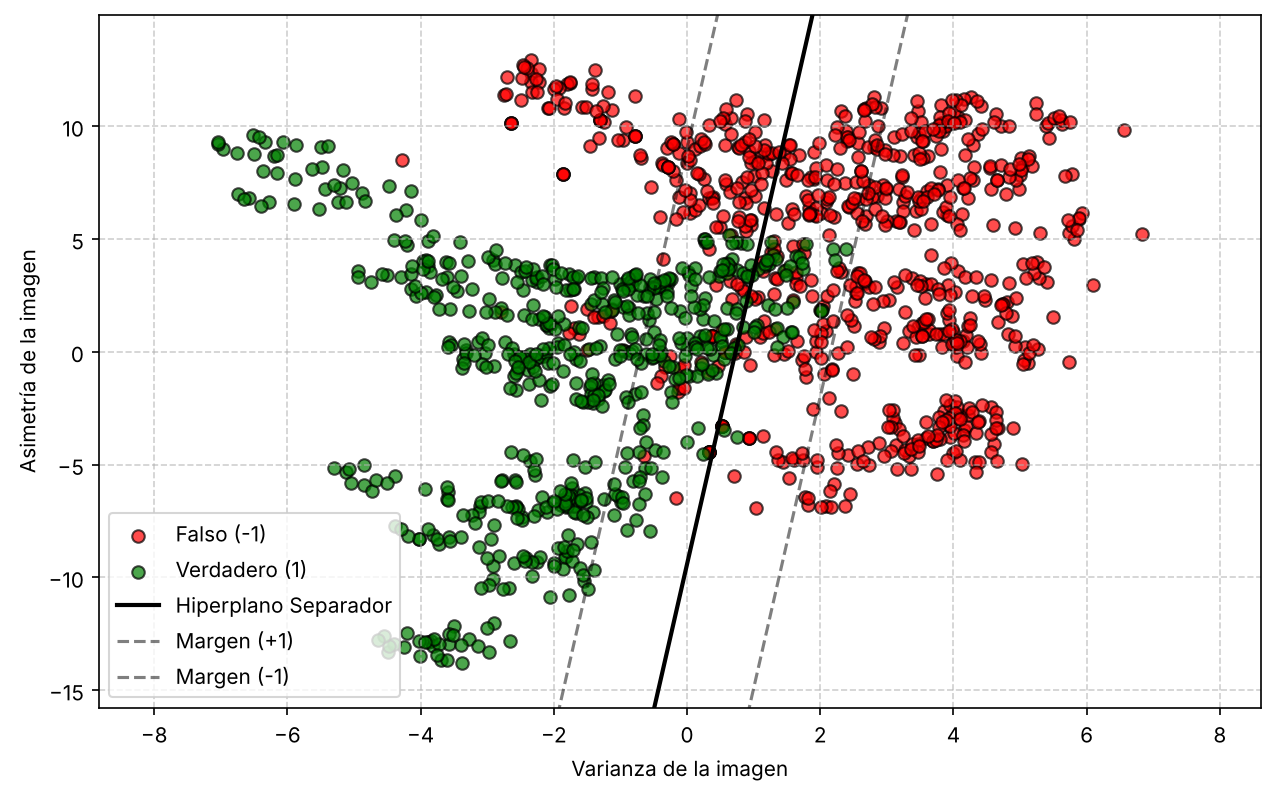
\includegraphics[width=0.8\textwidth]{svmpython.png}
    \caption{Frontera de decisión lineal y bordes del margen obtenidos para el conjunto de datos \textit{Banknote Authentication}, usando las variables varianza y asimetría.}
    \label{fig:svm_resultado}
\end{figure}

\begin{itemize}
    \item \textbf{El hiperplano de decisión:} la línea sólida es el conjunto $\{\mathbf{x} \in \mathbb{R}^2 \mid \mathbf{w}^T \mathbf{x} + b = 0\}$, donde la función de decisión cambia de signo. Divide el plano en las dos regiones de clasificación.

    \item \textbf{Bordes del margen:} las líneas discontinuas son las rectas $\mathbf{w}^T \mathbf{x} + b = 1$ y $\mathbf{w}^T \mathbf{x} + b = -1$. La distancia entre ellas es $\frac{2}{\|\mathbf{w}\|}$; el término de regularización empuja a que sea lo mayor posible.

    \item \textbf{Violaciones del margen ($\xi_i > 0$):} se observan puntos que invaden la banda del margen o que incluso quedan al otro lado del hiperplano. Esto es lo esperado al no ser los datos separables: el modelo acepta estas violaciones, con un coste regulado por $\lambda$, a cambio de un margen más amplio. Este compromiso entre error de entrenamiento y amplitud del margen tiende a mejorar la generalización y a reducir el sobreajuste al ruido de los datos.
\end{itemize}

\newpage
\subsection{Hard Margin (formulación dual)}

\subsubsection{Selección del Conjunto de Datos}

\noindent El conjunto de datos seleccionado es el clásico \textbf{Iris Dataset} de Ronald Fisher, del que tomamos únicamente las observaciones de las clases \textit{Iris Setosa} e \textit{Iris Versicolor}.

\begin{enumerate}
    \item \textbf{Dos características:} usamos el largo del sépalo y el largo del pétalo, de modo que $\mathcal{X} \subseteq \mathbb{R}^2$ y podemos representar gráficamente la frontera.

    \item \textbf{Etiquetas:} como en el margen suave, transformamos las etiquetas a $\mathcal{Y} = \{-1, 1\}$.

    \item \textbf{Separabilidad lineal:} Setosa es linealmente separable de las otras dos especies, y en particular de Versicolor. Al no haber solapamiento, el problema de margen duro es factible (todas las holguras son $\xi_i = 0$), hay dualidad fuerte y podemos resolverlo por la vía dual.
\end{enumerate}

\subsubsection{Desarrollo del Algoritmo: Optimización Dual}

\noindent Recordemos el problema dual en forma matricial. Por comodidad numérica lo escribimos como minimización (cambiando el signo del objetivo):
\[ \min_{\alpha} \; \frac{1}{2}\alpha^T Q \alpha - \mathbf{1}^T \alpha \quad \text{s.a.} \quad \mathbf{y}^T\alpha = 0, \quad \alpha \geq 0, \qquad Q = \mathrm{diag}(\mathbf{y})\,K\,\mathrm{diag}(\mathbf{y}). \]

\noindent \textbf{Importante:} el problema tiene \textit{dos} tipos de restricción. Las cotas $\alpha_i \geq 0$ son fáciles de imponer (basta con truncar los valores negativos), pero la restricción de igualdad $\sum_i \alpha_i y_i = 0$, que procede de la derivada respecto a $b$, no se conserva al truncar. Si se ignora, se está resolviendo en realidad el dual de una SVM \textit{sin sesgo}, y el $b$ calculado a posteriori no corresponde al problema planteado. Por ello resolvemos el dual con un optimizador que admite ambas restricciones: el método SLSQP (programación cuadrática secuencial) de \texttt{scipy}.

\vspace{0.2cm}
\noindent \textbf{1. Matriz de Gram e Inicialización}

\noindent La formulación dual solo necesita los productos escalares entre observaciones, así que calculamos de antemano la \textbf{Matriz de Gram} $K \in \mathbb{R}^{n \times n}$, con $K_{ij} = \mathbf{x}_i^T \mathbf{x}_j$. Al ser una matriz de Gram, es semidefinida positiva, y por tanto también lo es $Q$: el problema es convexo y cualquier óptimo local es global.

\noindent Las variables a optimizar ya no son $(\mathbf{w}, b)$, sino el vector de multiplicadores de Lagrange $\alpha \in \mathbb{R}^n$, que inicializamos en $\mathbf{0}$ (es un punto factible).

\begin{lstlisting}
import numpy as np
from sklearn.datasets import load_iris
from scipy.optimize import minimize

iris = load_iris()
X = iris.data[:100, [0, 2]]   # Setosa y Versicolor; largo de sepalo y de petalo
y = iris.target[:100]
y = np.where(y == 0, -1, 1).astype(float)

n_samples, n_features = X.shape

# Matriz de Gram y matriz Q del dual
K = X @ X.T
Q = np.outer(y, y) * K

# Punto inicial (factible)
alphas0 = np.zeros(n_samples)
\end{lstlisting}

\vspace{0.2cm}
\noindent \textbf{2. Resolución del Dual con Restricciones}

\noindent Proporcionamos al optimizador la función objetivo, su gradiente $Q\alpha - \mathbf{1}$, las cotas $\alpha_i \geq 0$ (condición KKT de factibilidad dual) y la restricción de igualdad $\mathbf{y}^T\alpha = 0$:

\begin{lstlisting}
def objetivo(a):
    return 0.5 * a @ Q @ a - a.sum()

def gradiente(a):
    return Q @ a - np.ones(n_samples)

restricciones = [{'type': 'eq',
                  'fun': lambda a: a @ y,    # sum_i alpha_i y_i = 0
                  'jac': lambda a: y}]
cotas = [(0, None)] * n_samples              # alpha_i >= 0

res = minimize(objetivo, alphas0, jac=gradiente,
               bounds=cotas, constraints=restricciones,
               method='SLSQP',
               options={'maxiter': 1000, 'ftol': 1e-12})
alphas = res.x
\end{lstlisting}

\vspace{0.2cm}
\noindent \textbf{3. Recuperación de $\mathbf{w}$ y $b$}

\noindent Una vez obtenido $\alpha$, la condición de estacionariedad nos da $\mathbf{w} = \sum_i \alpha_i y_i \mathbf{x}_i$. Para el sesgo usamos la holgura complementaria: los vectores de soporte ($\alpha_i > 0$) cumplen $y_i(\mathbf{w}^T\mathbf{x}_i + b) = 1$, de donde $b = y_i - \mathbf{w}^T\mathbf{x}_i$. Promediamos sobre todos ellos para reducir el efecto del error numérico.

\begin{lstlisting}
# Estacionariedad: w = sum_i alpha_i y_i x_i
w = (alphas * y) @ X

# Vectores de soporte (alpha_i > 0, con tolerancia numerica)
idx = np.where(alphas > 1e-6)[0]

# Holgura complementaria: b = y_s - w^T x_s, promediado
b = np.mean(y[idx] - X[idx] @ w)

# Comprobaciones de las condiciones KKT
print("Optimizacion correcta:", res.success)
print("sum alpha_i y_i =", alphas @ y)                 # ~ 0
print("min y_i f(x_i) =", np.min(y * (X @ w + b)))    # ~ 1
\end{lstlisting}

\noindent Las dos últimas líneas verifican numéricamente la restricción de igualdad del dual y la factibilidad primal: el mínimo de $y_i(\mathbf{w}^T\mathbf{x}_i + b)$ debe ser (aproximadamente) $1$, alcanzado en los vectores de soporte.

\subsubsection{Análisis Geométrico de Resultados y Frontera de Decisión}

\noindent La representación de la solución se muestra en la Figura \ref{fig:svm_hard_margin}.

\begin{figure}[h]
    \centering
    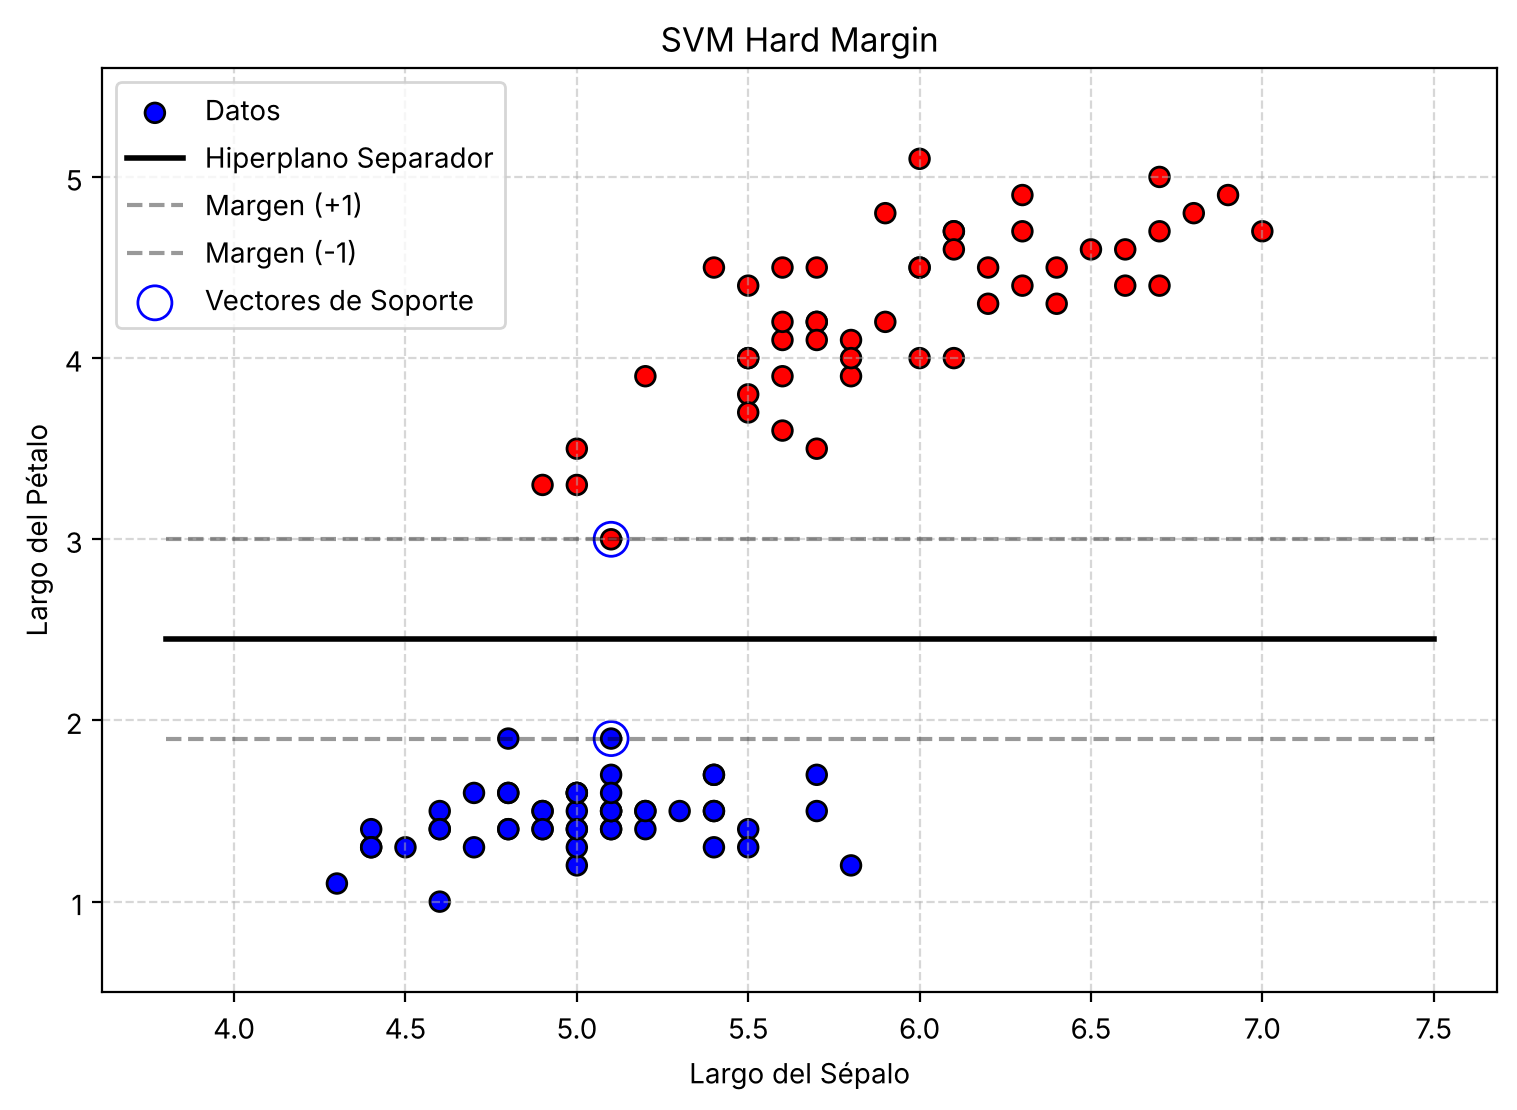
\includegraphics[width=0.8\textwidth]{diagrama2.png}
    \caption{Frontera de decisión de margen duro y vectores de soporte obtenidos mediante la formulación dual, para las clases Setosa y Versicolor del conjunto de datos \textit{Iris}.}
    \label{fig:svm_hard_margin}
\end{figure}

\noindent \textbf{Discusión:}
\begin{itemize}
    \item \textbf{Vectores de Soporte:} el vector $\mathbf{w}$ queda determinado por muy pocas muestras (las que tienen $\alpha_i > 0$). El resto tienen multiplicador nulo y no influyen en la frontera: podríamos eliminarlas del conjunto de entrenamiento y la solución no cambiaría.

    \item \textbf{Bordes del margen:} las rectas $\mathbf{w}^T \mathbf{x} + b = \pm 1$ delimitan la ``banda de seguridad'', de anchura $\frac{2}{\|\mathbf{w}\|}$. Al tratarse de margen duro, ningún punto queda dentro de la banda; lo comprobamos numéricamente con $\min_i y_i(\mathbf{w}^T\mathbf{x}_i + b) \approx 1$.

    \item \textbf{Holgura complementaria:} la condición $\alpha_i [y_i(\mathbf{w}^T \mathbf{x}_i + b) - 1] = 0$ implica que solo los puntos situados exactamente sobre los bordes del margen pueden tener $\alpha_i \neq 0$. En la figura se comprueba que los vectores de soporte marcados son precisamente puntos sobre las rectas discontinuas.
\end{itemize}

\subsubsection{Análisis del Código}
\paragraph{1. Selección y preparación de los datos}

\begin{lstlisting}
X = iris.data[:100, [0, 2]]
y = iris.target[:100]
y = np.where(y == 0, -1, 1).astype(float)
\end{lstlisting}

\begin{itemize}
    \item \textbf{Selección de clases (\texttt{:100}):} las 100 primeras observaciones del dataset corresponden a Setosa y Versicolor, un par de clases linealmente separable, que es lo que necesitamos para el margen duro.
    \item \textbf{Selección de características (\texttt{[0, 2]}):} nos quedamos con el largo del sépalo y el largo del pétalo, lo que permite representar la frontera en el plano.
    \item \textbf{Etiquetas (\texttt{np.where}):} aplica la biyección $0 \mapsto -1$, $1 \mapsto 1$, necesaria para que la restricción $y_i(\mathbf{w}^T \mathbf{x}_i + b) \geq 1$ valga para ambas clases. El \texttt{.astype(float)} evita problemas de tipos en las operaciones posteriores.
\end{itemize}

\paragraph{2. Dimensiones}

\begin{lstlisting}
n_samples, n_features = X.shape
\end{lstlisting}

\noindent El atributo \texttt{.shape} devuelve las dimensiones de la matriz de datos: \texttt{n\_samples} es el número de observaciones $n$, que coincide con la dimensión del vector $\alpha$, y \texttt{n\_features} es la dimensión $d$ del espacio de entrada.

\paragraph{3. Matriz de Gram y matriz $Q$}

\begin{lstlisting}
K = X @ X.T
Q = np.outer(y, y) * K
\end{lstlisting}

\noindent La primera línea calcula todos los productos escalares $\mathbf{x}_i^T\mathbf{x}_j$ de una vez, como el producto matricial $XX^T$. Su coste es $\mathcal{O}(n^2 d)$, igual que calcularlos uno a uno; la ventaja de la versión vectorizada es práctica (NumPy la ejecuta en código optimizado), no de complejidad. La segunda línea construye $Q_{ij} = y_i y_j K_{ij}$: \texttt{np.outer(y, y)} es la matriz $\mathbf{y}\mathbf{y}^T$ y \texttt{*} es el producto elemento a elemento. Para usar un kernel no lineal bastaría con sustituir $K$ por la matriz $K(\mathbf{x}_i, \mathbf{x}_j)$ correspondiente.

\paragraph{4. Optimizador y restricciones}

\begin{itemize}
    \item \textbf{Objetivo y gradiente:} \texttt{objetivo} es $\frac12\alpha^TQ\alpha - \mathbf{1}^T\alpha$ (el dual cambiado de signo) y \texttt{gradiente} es su gradiente exacto, $Q\alpha - \mathbf{1}$. Proporcionar el gradiente evita que el optimizador tenga que aproximarlo numéricamente.
    \item \textbf{Cotas:} \texttt{(0, None)} impone $\alpha_i \geq 0$ para cada $i$, la condición KKT de factibilidad dual.
    \item \textbf{Restricción de igualdad:} el diccionario con \texttt{'type': 'eq'} impone $\mathbf{y}^T\alpha = 0$, que procede de la condición de estacionariedad respecto a $b$.
\end{itemize}

\paragraph{5. Recuperación de $\mathbf{w}$ y $b$}

\begin{lstlisting}
w = (alphas * y) @ X
idx = np.where(alphas > 1e-6)[0]
b = np.mean(y[idx] - X[idx] @ w)
\end{lstlisting}

\begin{itemize}
    \item \textbf{Vector normal ($\mathbf{w}$):} por la condición de estacionariedad, $\mathbf{w} = \sum_i \alpha_i y_i \mathbf{x}_i$. El vector \texttt{alphas * y} contiene los coeficientes $\alpha_i y_i$ y al multiplicarlo por $X$ se obtiene exactamente esa combinación lineal de las filas de $X$.
    \item \textbf{Sesgo ($b$):} \texttt{np.where} selecciona los índices con $\alpha_i > 0$ (los vectores de soporte), con una tolerancia de $10^{-6}$ porque numéricamente los multiplicadores nulos salen como valores muy pequeños, no como ceros exactos. Para ellos se cumple $y_i(\mathbf{w}^T\mathbf{x}_i + b) = 1$, luego $b = y_i - \mathbf{w}^T\mathbf{x}_i$. Promediar con \texttt{np.mean} reduce el efecto de los errores de redondeo.
\end{itemize}

\paragraph{6. Representación gráfica en $\mathbb{R}^2$}

\begin{lstlisting}
if abs(w[1]) > 1e-9:
    y_plot = -(w[0] * x_plot + b) / w[1]
    y_margen_pos = -(w[0] * x_plot + b - 1) / w[1]
    y_margen_neg = -(w[0] * x_plot + b + 1) / w[1]
\end{lstlisting}

\noindent Para dibujar la recta $\mathbf{w}^T \mathbf{x} + b = 0$ la escribimos en coordenadas, $w_1 x_1 + w_2 x_2 + b = 0$, y despejamos $x_2$ en función de $x_1$:
\[ x_2 = \frac{-(w_1 x_1 + b)}{w_2} \]
La condición \texttt{abs(w[1]) > 1e-9} evita dividir por cero cuando la recta es vertical ($w_2 = 0$). Los bordes del margen se obtienen igual, sustituyendo el $0$ del lado derecho por $+1$ y $-1$.

\newpage
%=====================================================================
\section{Fundamentos de Computación Cuántica}
%=====================================================================

\noindent En esta sección se establecen las bases teóricas de la computación cuántica, partiendo de una comparativa directa con los sistemas de información clásicos. Se sigue el curso \textit{Understanding Quantum Information and Computation} de IBM Quantum \cite{watrous2024understanding}.

\subsection{Sistemas individuales}
\subsubsection{Información Clásica}

\paragraph{Estados clásicos y vectores de probabilidad}\mbox{}\\

\noindent Supongamos que tenemos un sistema que almacena información. Asumimos que este sistema puede estar en uno de un número finito de \textit{estados clásicos} (configuraciones que pueden reconocerse y describirse sin ambigüedad) en cada instante.

\noindent Llamaremos $X$ al sistema y usaremos el símbolo $\Sigma$ para referirnos al conjunto de estados clásicos de $X$. Asumimos que $\Sigma$ es un conjunto finito y no vacío. Algunos ejemplos:
\begin{itemize}
    \item Si $X$ es un bit, entonces $\Sigma = \{0, 1\}$, conjunto al que nos referimos como el \textit{alfabeto binario}.
    \item Si $X$ es un dado de seis caras, entonces $\Sigma = \{1, 2, 3, 4, 5, 6\}$.
    \item Si $X$ es el interruptor de un ventilador eléctrico, entonces $\Sigma = \{\text{alto, medio, bajo, apagado}\}$.
\end{itemize}

\noindent A menudo representamos nuestro conocimiento sobre el estado de $X$ asociando probabilidades a sus posibles estados clásicos, lo que llamaremos un \textbf{estado probabilístico}. Por ejemplo, si $X$ es un bit, podríamos creer que está en el estado $0$ con probabilidad $3/4$ y en el estado $1$ con probabilidad $1/4$:
\[ \Pr(X = 0) = \frac{3}{4} \quad \text{y} \quad \Pr(X = 1) = \frac{1}{4}. \]

\noindent Otra forma de representar este estado probabilístico es mediante un vector columna:
\[ \begin{pmatrix} 3/4 \\ 1/4 \end{pmatrix}. \]
\noindent La probabilidad del $0$ va en la entrada superior y la del $1$ en la inferior, siguiendo el orden convencional de $\{0, 1\}$.

\noindent En general, cualquier estado probabilístico se representa mediante un vector columna que satisface:
\begin{enumerate}
    \item Todas las entradas son números reales no negativos.
    \item La suma de las entradas es igual a 1.
\end{enumerate}

\noindent Recíprocamente, cualquier vector columna con estas dos propiedades representa un estado probabilístico. A estos vectores los llamaremos \textbf{vectores de probabilidad}.

\paragraph{Medición de estados probabilísticos}\mbox{}\\

\noindent Por \textit{medir} un sistema entendemos observarlo y reconocer sin ambigüedad el estado clásico en el que se encuentra.

\noindent Al medir, cambia nuestro conocimiento del sistema y, por tanto, el estado probabilístico que le asociamos. Si reconocemos que $X$ está en el estado clásico $a \in \Sigma$, el nuevo vector de probabilidad tiene un 1 en la entrada correspondiente a $a$ y 0 en todas las demás. Denotamos este vector por $|a\rangle$ (``ket $a$''), y a los vectores de este tipo se les llama \textbf{vectores de la base estándar}.

Por ejemplo, si el sistema es un bit:
\[ |0\rangle = \begin{pmatrix} 1 \\ 0 \end{pmatrix} \quad \text{y} \quad |1\rangle = \begin{pmatrix} 0 \\ 1 \end{pmatrix}. \]

Cualquier vector columna puede expresarse como combinación lineal de los vectores de la base estándar. Por ejemplo:
\[ \begin{pmatrix} 3/4 \\ 1/4 \end{pmatrix} = \frac{3}{4}|0\rangle + \frac{1}{4}|1\rangle. \]

Para ilustrar el cambio de estado al medir, supongamos que lanzamos una moneda equilibrada y la tapamos antes de mirarla. Su estado probabilístico es:
\[ \begin{pmatrix} 1/2 \\ 1/2 \end{pmatrix} = \frac{1}{2}|\text{cara}\rangle + \frac{1}{2}|\text{cruz}\rangle. \]

Si destapamos la moneda y vemos cruz, actualizamos nuestra descripción a $|\text{cruz}\rangle$. Si volvemos a taparla y destaparla, seguirá siendo cruz, lo cual es coherente con el vector $|\text{cruz}\rangle$.

Aunque esto parezca trivial en el caso clásico, los sistemas cuánticos se comportan de forma análoga respecto a la medición, y tener presente esta analogía ayuda a que la información cuántica parezca menos extraña.

\begin{tcolorbox}[colback=blue!5!white,colframe=blue!75!black,title=\textbf{Aclaración: El cambio de estado tras la medición}]
Un estado probabilístico describe nuestro \textbf{conocimiento} sobre el sistema. En el caso de la moneda, mirar no cambia la moneda: ya era cruz debajo de la mano. Lo que cambia es nuestra información, y con ella el vector, que pasa de $\frac{1}{2}|\text{cara}\rangle + \frac{1}{2}|\text{cruz}\rangle$ a $|\text{cruz}\rangle$. Otra persona que no haya mirado seguiría describiendo la moneda con el vector original.

\textbf{El salto a la cuántica:} en el caso cuántico, la regla de actualización tras medir es formalmente la misma: el estado pasa a ser $|a\rangle$. La diferencia está en que las amplitudes cuánticas \textbf{no pueden interpretarse} simplemente como probabilidades que reflejan nuestra ignorancia. Son números complejos que, al aplicar operaciones, pueden \textbf{interferir}: sumarse o cancelarse entre sí. Las probabilidades clásicas, al ser no negativas, nunca se cancelan. Este fenómeno de interferencia, que veremos con operaciones como la de Hadamard, no tiene análogo clásico.
\end{tcolorbox}

\subsubsection{Información Cuántica}

\paragraph{Estados Cuánticos y Qubits}\mbox{}\\

\noindent A diferencia de la información clásica, la \textbf{información cuántica} utiliza números complejos para describir el estado del sistema. El estado cuántico de un sistema se representa mediante un vector columna con las siguientes propiedades:
\begin{enumerate}
    \item Las entradas son \textbf{números complejos} (llamados amplitudes).
    \item La suma de los \textbf{módulos al cuadrado} de las entradas es igual a 1.
\end{enumerate}

Es decir, un estado cuántico es un vector unitario respecto a la norma euclídea compleja: si $v = (\alpha_1, \dots, \alpha_n)^T$, entonces $\|v\| = \sqrt{\sum_{k=1}^n |\alpha_k|^2} = 1$. El análogo cuántico del bit clásico se denomina \textbf{qubit}, y sus estados de la base estándar se denotan por $|0\rangle$ y $|1\rangle$. Un qubit también puede encontrarse en estados de \textbf{superposición}, como:
\begin{itemize}
    \item \textbf{Estados más/menos:} $|+\rangle = \frac{1}{\sqrt{2}}|0\rangle + \frac{1}{\sqrt{2}}|1\rangle$ \quad y \quad $|-\rangle = \frac{1}{\sqrt{2}}|0\rangle - \frac{1}{\sqrt{2}}|1\rangle$.
    \item \textbf{Estado con amplitudes complejas:} por ejemplo $|\psi\rangle = \frac{1+2i}{3}|0\rangle - \frac{2}{3}|1\rangle$.
\end{itemize}

El vector fila (\textit{bra}) asociado a $|\psi\rangle$ es su \textbf{transpuesta conjugada}, $\langle\psi| = |\psi\rangle^\dagger$: se transpone el vector y se conjugan todas sus entradas. Por ejemplo:
\[ \text{Si } |\psi\rangle = \begin{bmatrix} \frac{1+2i}{3} \\ -\frac{2}{3} \end{bmatrix}, \quad \text{entonces } \langle \psi | = \begin{bmatrix} \frac{1-2i}{3} & -\frac{2}{3} \end{bmatrix}. \]

\paragraph{Medición de Estados Cuánticos}\mbox{}\\

\noindent Al medir un estado cuántico en la base estándar, se obtiene uno de los estados clásicos (en un qubit, $0$ o $1$) y el estado pasa a ser el vector de la base estándar correspondiente. A diferencia del caso clásico, las entradas del vector no son probabilidades sino amplitudes complejas. La \textbf{regla de Born} establece que la probabilidad de obtener un estado clásico es el \textbf{módulo al cuadrado} de la amplitud correspondiente.

\begin{tcolorbox}[colback=gray!5!white,colframe=gray!75!black,title=\textbf{Ejemplo: Medición de un estado con amplitudes complejas}]
Supongamos que medimos el estado $|\psi\rangle = \frac{1+2i}{3}|0\rangle - \frac{2}{3}|1\rangle$. Para hallar las probabilidades, calculamos el módulo al cuadrado ($|\alpha|^2 = \alpha \cdot \overline{\alpha}$, donde $\overline{\alpha}$ es el conjugado):
\begin{itemize}
    \item $\Pr(\text{resultado } 0) = \left| \frac{1+2i}{3} \right|^2 = \left( \frac{1+2i}{3} \right) \left( \frac{1-2i}{3} \right) = \frac{1 - (-4)}{9} = \frac{5}{9}$
    \item $\Pr(\text{resultado } 1) = \left| -\frac{2}{3} \right|^2 = \frac{4}{9}$
\end{itemize}
Como corresponde a un estado cuántico válido, $\frac{5}{9} + \frac{4}{9} = 1$.
\end{tcolorbox}

\paragraph{Operaciones Unitarias y Puertas Cuánticas}\mbox{}\\

\noindent En mecánica cuántica, las operaciones sobre un sistema aislado no se describen mediante matrices estocásticas, sino mediante \textbf{matrices unitarias}.

Una matriz cuadrada $U$ con entradas complejas es unitaria si:
\[ U^\dagger U = \mathbb{I} = U U^\dagger \]
donde $U^\dagger$ es la transpuesta conjugada de $U$ e $\mathbb{I}$ la identidad. Equivalentemente, $U$ preserva la norma euclídea ($\|Uv\| = \|v\|$ para todo $v$), lo que garantiza que un estado cuántico se transforma en otro estado cuántico y las probabilidades siguen sumando 1. Algunas operaciones unitarias fundamentales sobre un qubit son:

\begin{itemize}
    \item \textbf{Operaciones de Pauli:}
    \[
    I = \begin{bmatrix} 1 & 0 \\ 0 & 1 \end{bmatrix}, \quad
    X = \sigma_x = \begin{bmatrix} 0 & 1 \\ 1 & 0 \end{bmatrix}, \quad
    Y = \sigma_y = \begin{bmatrix} 0 & -i \\ i & 0 \end{bmatrix}, \quad
    Z = \sigma_z = \begin{bmatrix} 1 & 0 \\ 0 & -1 \end{bmatrix}
    \]
    La puerta $X$ es un \textit{bit flip} (análogo al NOT clásico: $X|0\rangle = |1\rangle$, $X|1\rangle = |0\rangle$) y la puerta $Z$ un \textit{phase flip} ($Z|0\rangle = |0\rangle$, $Z|1\rangle = -|1\rangle$).

    \item \textbf{Operación de Hadamard ($H$):}
    \[ H = \begin{bmatrix} \frac{1}{\sqrt{2}} & \frac{1}{\sqrt{2}} \\ \frac{1}{\sqrt{2}} & -\frac{1}{\sqrt{2}} \end{bmatrix} \]
    Cumple $H|0\rangle = |+\rangle$ y $H|1\rangle = |-\rangle$. Además, $H|+\rangle = |0\rangle$: las amplitudes de $|1\rangle$ se cancelan. Este es un primer ejemplo de interferencia.

    \item \textbf{Operaciones de Fase ($P_\theta$):}
    Multiplican la amplitud de $|1\rangle$ por una fase $e^{i\theta}$:
    \[ P_\theta = \begin{bmatrix} 1 & 0 \\ 0 & e^{i\theta} \end{bmatrix} \]
    Casos particulares de gran utilidad son la puerta $S = P_{\pi/2}$ y la puerta $T = P_{\pi/4}$.
\end{itemize}

La composición de operaciones unitarias se representa mediante el producto de matrices (aplicar primero $U_1$ y luego $U_2$ corresponde a $U_2 U_1$). Por ejemplo, la operación $HSH$ es una \textbf{raíz cuadrada de NOT}: aplicada dos veces equivale a la puerta $X$:
\[ (HSH)^2 = \begin{bmatrix} \frac{1+i}{2} & \frac{1-i}{2} \\ \frac{1-i}{2} & \frac{1+i}{2} \end{bmatrix}^2 = \begin{bmatrix} 0 & 1 \\ 1 & 0 \end{bmatrix} = X \]

%=====================================================================
\newpage
\bibliographystyle{plain}
\bibliography{referencias}

\end{document}
